\documentclass[11pt,a4paper]{book}

\usepackage{latexsettings} % Verweis auf Datei latexsettings.sty
\usepackage{custom_commands}

% Titelseite
\title{Grundlagen der Fachdidaktik Physik}
\author{Axel Enders}
\date{\today}

\begin{document}

% Titelseite generieren
\begin{titlepage}
    \newgeometry{left=2.5cm, right=2.5cm, top=2.5cm, bottom=2.5cm} %andere Seitengeometrie fr Titelseite 5.8.24 J.Hlawatsch
	\vs{0.5cm}
	\begin{figure}[h]
	\centering
	
\includegraphics[scale=.1]{Logo_physikdidaktik_long.png}
	% \caption{Meine Grafik}
	\label{fig:Logo}
	\end{figure}
	
	\vs{1cm}
	\begin{center}
	\Large \textbf{Bayreuther}
	\bip\bip
	\Huge \textbf{Abiturtrainer \\ Astrophysik}
	\bip\bip
	\Large
	(Stand Februar 2025)
	\end{center}

	\vs{6cm}

%	\begin{flushright}
%		\textbf{Apl. Prof. Dr. Stefan Hilger} \\
%			Didaktik der Mathematik  \\
%			Katholische Universitaet Eichst\"att-Ingolstadt \\
%			Ostenstrasse 26 - 28  \\
%			85071 Eichst\"att \\
%			Stefan.Hilger@ku.de \\
%
%	\vs{0.5cm}
%
%		\textbf{Prof. Dr. Axel Enders} \\
%		\textbf{Julius B. Hlawatsch, M.Sc., M.Ed.}\\
%		Lehrstuhl f\"ur Experimentalphysik XI und Didaktik der Physik  \\
%		Universit\"at Bayreuth  \\
%		Universit\"atstrasse 30  \\
%		95440 Bayreuth  \\
%		axel.enders@uni-bayreuth.de
%	\end{flushright}

\end{titlepage}

%---------------------------------------------------------------------------------------------------------------------------------
\newgeometry{left=2.5cm, right=2.5cm, top=2.5cm, bottom=2.5cm} %andere Seitengeometrie fr Vorwort und ToC 5.8.24 J.Hlawatsch
%---------------------------------------------------------------------------------------------------------------------------------
\newpage

\vs{3cm}
\section*{Vorwort}

\lipsum[2]

\vfill
\textbf{Hinweis zum Sprachgebrauch:} \\
Uns liegt die gleichsame Ansprache und Einbindung aller Menschen, unabhängig von ihrer Geschlechtsidentität, sehr am Herzen. In diesem Skript verwenden wir dennoch das generische Maskulinum für Personen aller Geschlechtsidentitäten. Wir haben uns für diese Lösung entschieden, da sie für uns die beste ist, um die Lesbarkeit zu gewährleisten und den Vorgaben der Bayerischen Staatsregierung zu entsprechen.



% Inhaltsverzeichnis
\tableofcontents
\newpage

\restoregeometry % nutze ab jetzt Notizenrand rechts 5.8.24 J.Hlawatsch

%\begin{ziele}
%	Hier stehen Ziele	
%\end{ziele}


\chapter{Abituraufgabe 2024-1}\label{Denk}

\begin{aufgabe}
	\textbf{1. Aufgabenname}
	\begin{enumerate}
		\item Unteraufgabe \hfill K3, S2 / I
		\item Unteraufgabe \hfill K3, S2 / I
	\end{enumerate}
	Zwischentext
	\begin{enumerate}[resume]
		\item Unteraufgabe \hfill K3, S2 / I
	\end{enumerate}
\end{aufgabe}


\section{Fachliche Grundlagen}

\section{Musterlösung}

\begin{hinweis}
	Hinweise werden so gesetzt.
\end{hinweis}


\newgeometry{left=2.5cm, right=2.5cm, top=2.5cm, bottom=2.5cm} %ab jetzt wieder ohne Notizenrand
% Literaturverzeichnis
\printbibliography

\appendix
\chapter{Teilkompetenzen der KMK-Bildungsstandards}\label{A_kmk}
aus: ISB. Gute Aufgaben im Physikunterricht – erkennen – einsetzen – erstellen –. Kompetenzorientierter Unterricht am Gymnasium. München 2023.
\includepdf[pages=7]{ISB_Gute_Aufgaben_im_Physikunterricht}

\chapter{Verblisten für Operationalisierte Lernziele}\label{A_Verbliste}
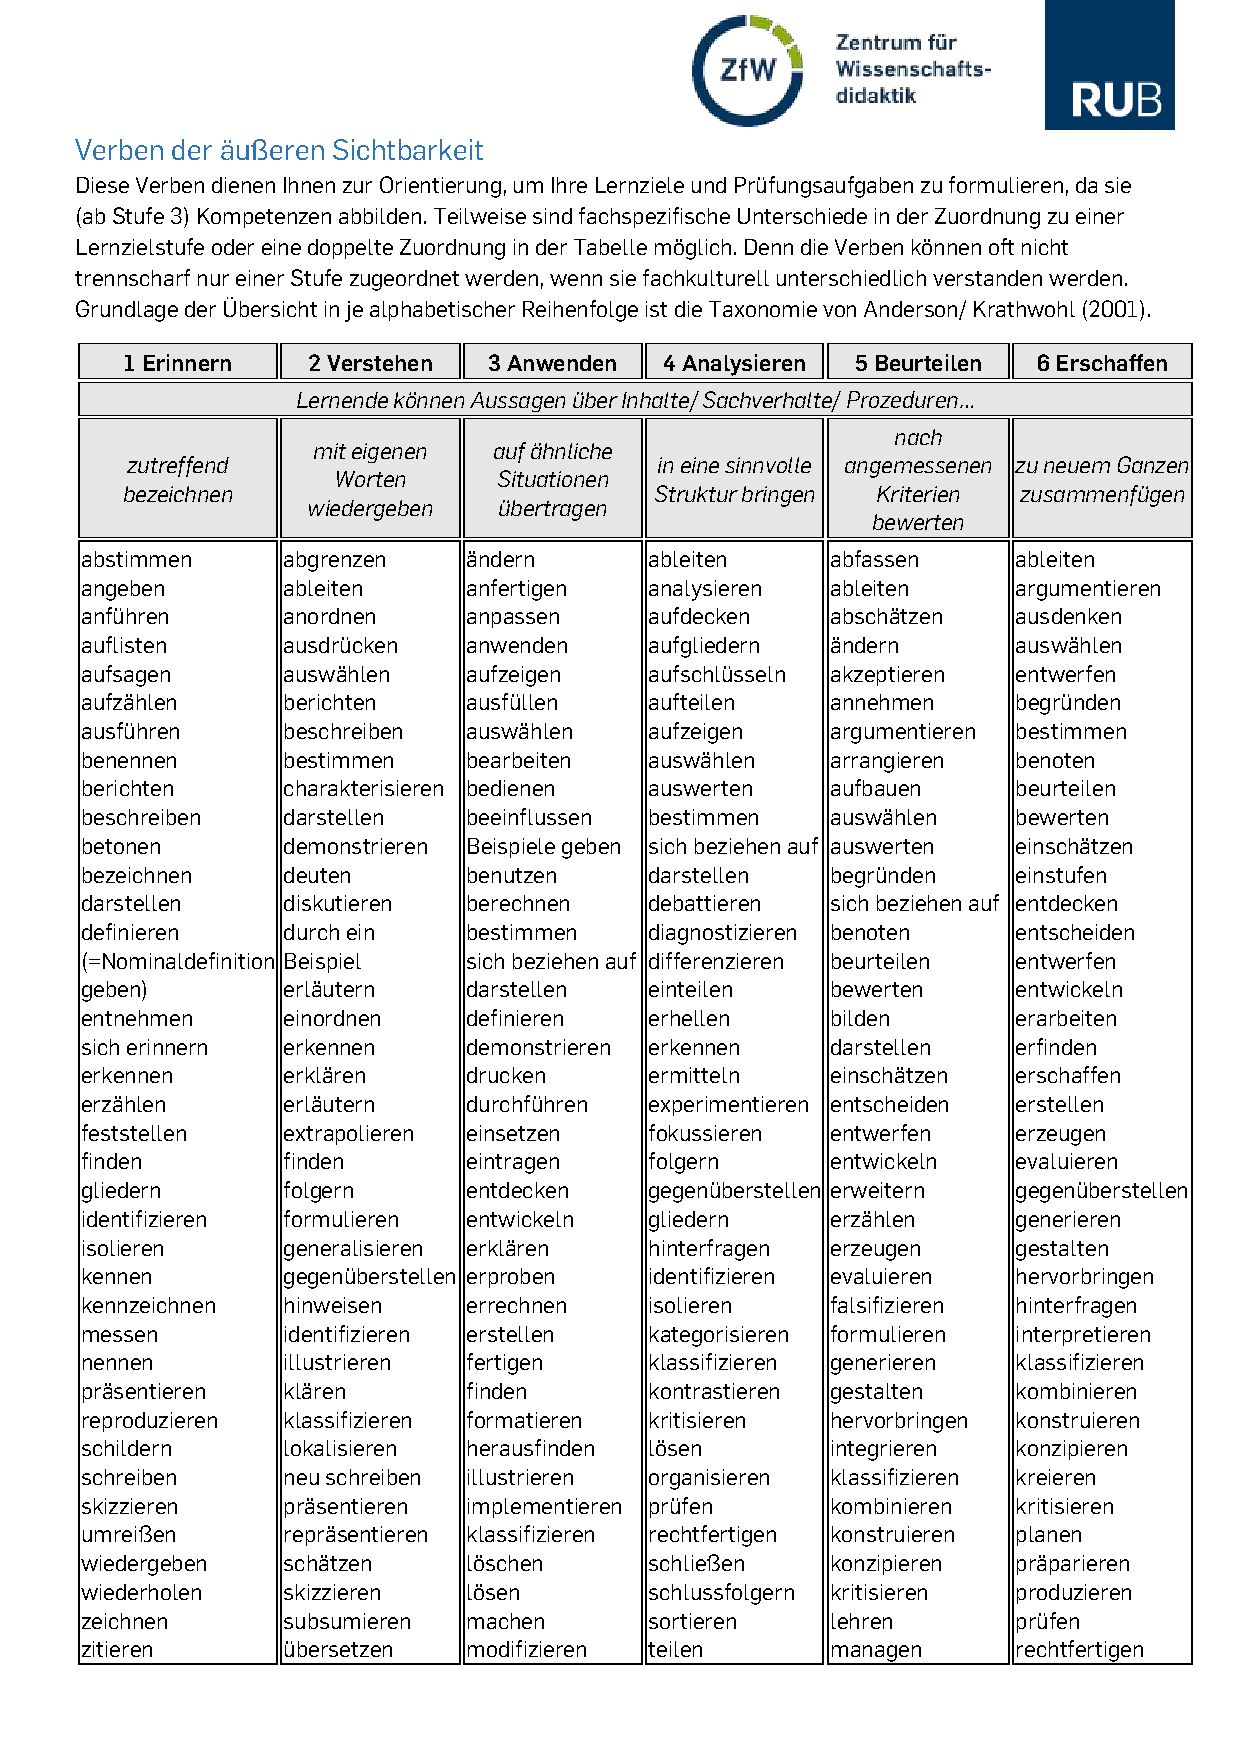
\includepdf[pages={1-2}]{Bilder/Verblisten_Kompetenz}

\chapter{Berliner Modell}\label{A_BerlinerModell}

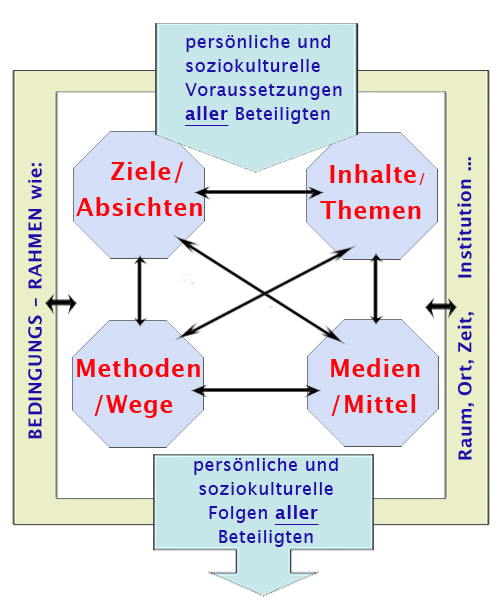
\includegraphics[width=10cm]{BerlinerModell1.jpg} \\
Bildquelle: \url{https://commons.wikimedia.org/wiki/File:BerlinerModell1.jpg}

\chapter{Weitere Artikulationsschemata}

\section{Grob-Phasen gem\"{a}{\ss} \textcite{DuitHausslerKircher}}
\begin{enumerate}
	\item {\bf Motivation} oder Einstiege
	\item {\bf Erarbeitung} Probleml\"{o}sung (beispielsweise im Experiment)
	\begin{enumerate}
	\item
	Planung des Experiments
	\item
	Durchf\"{u}hrung des Experiments
	\item
	Auswertung des Experiments
	\item
	R\"{u}ckblickende Er\"{o}rterung des Experiments
	\item
	Allgemeine Er\"{o}rterung
	\end{enumerate}
	\item {\bf Vertiefung} Integration, Behalten, Transfer.
\end{enumerate}

\section{\textcite{Ploeger}: Forschender Physikunterricht}
Konkret, anwendungsnah und auf den Punkt gebracht wird dieses Konzept in
\textcite{Ploeger} beschrieben.
Es finden sich dort auch viele Beispiele.
\begin{enumerate}
	\item {\bf Problemfrage}
	\item {\bf Vermutung}
	\item {\bf Versuchsplanung}
	\item {\bf Experiment}
	\item {\bf Auswertung}
\end{enumerate}
Der zentrale Unterschied zu Mothes ist die Sichtweise, aus der sie ihre Schemata formulieren. Während Mothes eher lehrerzentriert argumentiert, betont Plöger die aktive Beteiligung der Schüler an der Erarbeitung des Wissens.

\section{H.F.\ Bauer: Experimentalunterricht (1984)}
Das Grundschema des entdeckenden Unterrichts wird
hier spezialisiert-differenziert im Hinblick auf
das Experimentieren umgesetzt.

\mip Ziel des Unterrichts ist nicht Forschung an sich, sondern eine
Vertrautheit mit dem Forschen an sich.
	\begin{enumerate}
	\item {\bf Motivation}
	\item {\bf Problemherstellung}
	\item {\bf Meinungsbildung}
	\item {\bf Planen} und Konstruieren
	\item {\bf Laborieren --- Experimentieren}
	\item {\bf Schlie{\ss}en}
	\item {\bf Abstrahieren}
	\item {\bf Wissenssicherung durch Anwendung und \"{U}bung}
\end{enumerate}


\chapter{Beispiel einer didaktischen Analyse}\label{A_DidAna}

\end{document}